\section{Theoretical Introduction}

``Computational Neuroscience is an approach to understanding the information content of neural signals by modeling the nervous system at many different structural scales, including the biophysical, the circuit, and the systems levels. Computer simulations of neurons and neural networks are complementary to traditional techniques in neuroscience.'' \cite[Series Foreword]{dayan}

Understanding how the brain works is one of the hardest challenges the humanity has ever faced, and it is crucial in the progress of Science: understanding intelligence, the learning process and consciousness would be groundbreaking for the developing of new technologies. The main issue in  the study of the brain right now is retrieving the data: we now have enough computational power to process signals from millions of neurons at the same time, but we can't just put an electrode in everyone of them, although some are going in that direction \cite{neuralink}.

\myparagraph{Simulations} 
A less invasive solution is to use our knowledge of the brain to build complex, biologically plausible simulations of the brain, or parts of the brain, and we could retrieve from them all the data that is needed. 

However, this approach, deeply analyzed in the past \cite{smolensky}, doesn't offer assurance that the simulation and the real process could actually be interchangeable. In the present, many of the challenges of that time were overcome, in particular computational power \cite{bluegene}, and simulations are used to confirm theoretical models of the brain \cite{pellonisz}.

Still, finding the precise values for all the parameters of neurons in a big model is challenging and time consuming, therefore here is proposed a framework able to autonomously optimize the parameters of a given model, so that a selected output of the simulation will coincide with the desired one. In this case the model, that will be described in more detail later,  is an hypothetical column of the sensory cortex of a mammal, developed by Potjans \cite{potjans}, and the output is the firing rate of the excitatory neurons in four different layers. 

\myparagraph{Optimization} 
As it is being showed in other domains, such as predicting protein structure \cite{alphafold}, Deep Reinforcement Learning is well suited to learn complex features of models and act to modify them in a desired direction. In this work the algorithm selected has been a modified version of Deep Deterministic Policy Gradient \cite{lillicrap}, whose functioning will be explained in the next section.


\subsection{Reinforcement Learning} 

Reinforcement Learning is an area of machine learning which considers a setup consisting of an agent interacting with an environment through actions. The agent receives an input from the environment, chooses an action and receives a reward, based on the state of the environment after the action.
The agent behavior is defined by a policy, which maps actions to states. An action-value function tries to predict the reward after taking an action.

\begin{figure}[h]
	\centering
	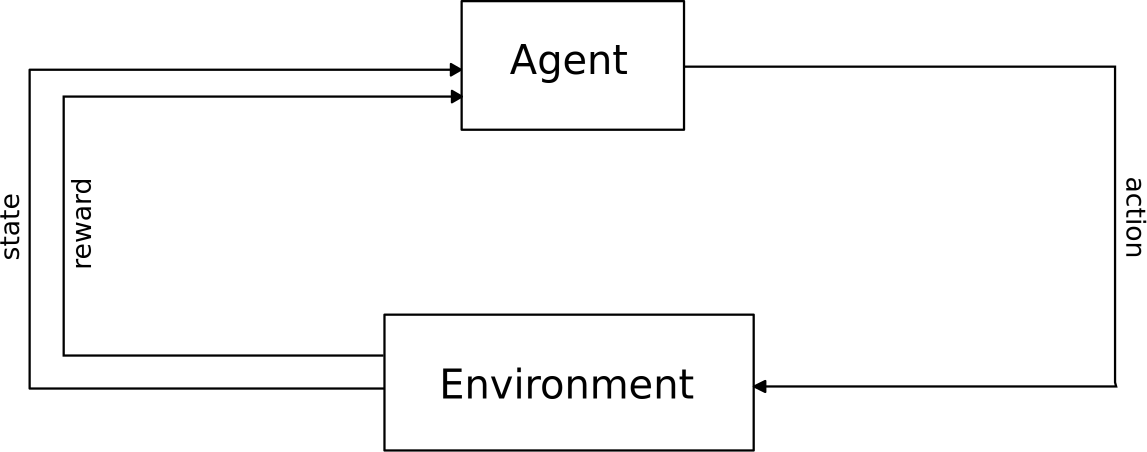
\includegraphics[scale=0.5]{pictures/rl.pdf}
	\caption{A Generic Reinforcement Learning setup}
	\label{fig:rl}
\end{figure}

\myparagraph{Bandits} 
We consider the simple case of the multi-armed bandit, where the environment reaches the terminal state after one single transition, and the agent has to choose a value for many different actions in a continuous space. The main problem to solve in this kind of setup is the balance between exploration and exploitation: we want the agent to take the best action possible action, but that could prevent him to explore the environment and find even better actions. One solution is to add simple Gaussian Noise to the actions, that decays slowly as the training goes on. This way the agent is able to point in one direction, but can choose a precise value only after a high number of episodes, when he has explored the environment enough.

\myparagraph{The Actor-Critic} 
The kind of algorithm we are using belongs to the family of actor-critic algorithms, where the actor is an Artificial Neural Network (ANN) that represents the policy, while the critic is another ANN representing the action-value function.
The critic is trained to predict how big the reward will be after an action is taken, and the actor is trained to take the best possible action. The critics try to understand the environment, and the actor uses this knowledge to change it in the desired way. It is useful to use ANNs because they are great at approximating functions, and since the environment we'll be using is very complex, they compensate the need to explore every possible combination of the parameters, inferring how the environment could respond in non-explored states.

\subsection{The Potjans and Diesmann Model} 

Potjans and Diesmann developed a model of a generic cortical column \cite{potjans}, extending the random balanced network \cite{brunel} to a four-layered column comprising excitatory and inhibitory populations. Biological data from in vivo observations on different mammals were used to infer the parameters. They simulated the resting state input from other cortical regions through a Poisson distribution.
The firing rates were compared with the values recorded on other studies \cite{kock} and the trend showed in both cases was similar (Figure \ref{fig:potjans_barplot}), yet it wasn't accurately matched. From the experiment it is apparent how much the structure of the model is prominent in defining its behavior.

\begin{figure}[h]
	\raggedleft
	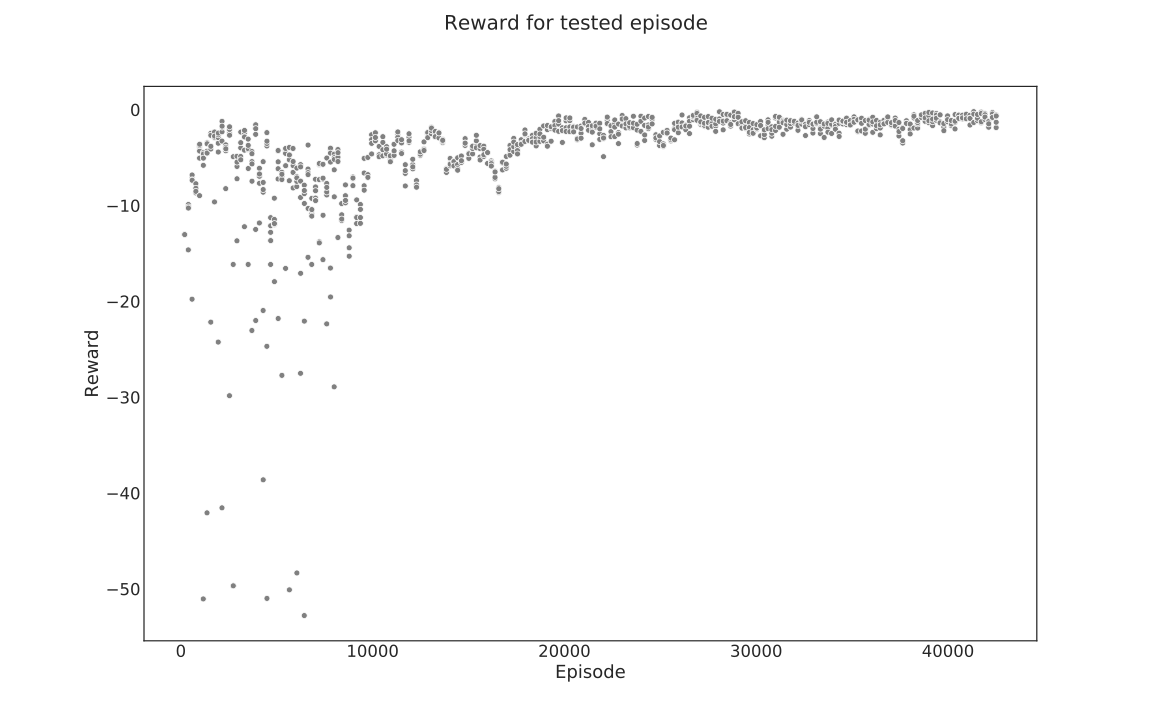
\includegraphics[scale=0.4]{pictures/potjans_barplot.pdf}
	\caption{Comparison of firing rates from the different studies}
	\label{fig:potjans_barplot}
\end{figure}

